\documentclass{standalone}
 
% Required packages

\usepackage{pgfplots}
\usetikzlibrary{arrows.meta}

\pgfplotsset{compat = newest}
\begin{document}
\tikzstyle{arrow} = [-{Latex[length=1.5mm, width=1mm]},align=flush center, font=\tiny, semithick]%
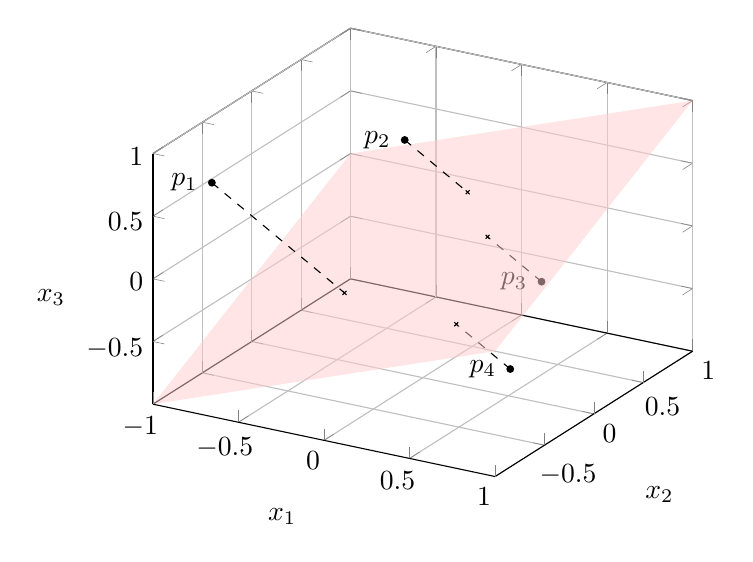
\begin{tikzpicture}
    

\begin{axis}[
    view = {30}{30},
    xlabel=$x_1$, ylabel=$x_2$, zlabel=$x_3$,
    z label style={rotate=-90},
    xmax=1,
    xmin=-1,
    ymax=1,
    ymin=-1,
    zmax=1,
    zmin=-1,
    % xtick={-0.5, 0.0, 0.5},
    ytick={-0.5, 0.0, 0.5, 1},
    ztick={-0.5, 0.0, 0.5, 1.0},
    grid
    ]

    \coordinate (p3) at (0.55, 0.25, -0.2);
    \node[label={180:{$p_3$}},circle,fill,inner sep=1pt] at (p3) {};
    \draw[thin, dashed] (p3) -- (0.35, 0.05, 0.2 );
    \addplot3[only marks, mark size=1pt, mark=x]  coordinates {(0.35, 0.05, 0.2 )};

    \coordinate (p4) at (0.8, -0.5, -0.45);
    \node[label={180:{$p_4$}},circle,fill,inner sep=1pt] at (p4) {};
    \draw[thin, dashed] (p4) -- (0.6, -0.7, -0.05);
    \addplot3[only marks, mark size=1pt, mark=x]  coordinates {(0.6, -0.7, -0.05)};

% plane
    \addplot3 [surf, draw opacity=0.0, fill=red!20, fill opacity=0.5] coordinates 
        {

            (-1,-1,-1) (-1, 1, 0) 
            
            (1, -1, 0) (1, 1, 1)

            };

    \coordinate (p1) at (-0.8, -0.75, 0.7);
    \node[label={180:{$p_1$}},circle,fill,inner sep=1pt] at (p1) {};
    \draw[thin, dashed] (p1) -- (-0.30833333, -0.25833333, -0.28333333);
    \addplot3[only marks, mark size=1pt, mark=x]  coordinates {(-0.30833333, -0.25833333, -0.28333333)};

    \coordinate (p2) at (-0.25, 0.25, 0.7);
    \node[label={180:{$p_2$}},circle,fill,inner sep=1pt] at (p2) {};
    \draw[thin, dashed] (p2) -- (-0.01666667, 0.48333333, 0.23333333);
    \addplot3[only marks, mark size=1pt, mark=x]  coordinates {(-0.01666667, 0.48333333, 0.23333333)};

    





        
        
 
\end{axis}


 
\end{tikzpicture}
 
\end{document}